% !TEX encoding = UTF-8
% !TEX TS-program = pdflatex
% !TEX root = ../main.tex
% !TEX spellcheck = it-IT

\documentclass[final, 11pt, a4paper, titlepage]{article}
\makeatletter
\AtBeginDocument{\let\hl\@firstofone}
\makeatother

\usepackage[italian]{babel}
\usepackage[utf8]{inputenc}
\usepackage[hidelinks]{hyperref}
\usepackage{graphicx}
\usepackage{textcomp}
\usepackage{wallpaper}
\usepackage{color}
\usepackage{mathtools}
\usepackage{amssymb}
\usepackage[
	backend=biber,
	citestyle=numeric-comp,
	hyperref,
	backref,
	sorting=none
]{biblatex}

\graphicspath{{images/}}

\addbibresource{bibliography.bib}


\defbibheading{bibliography}
{
    \phantomsection 
    \addcontentsline{toc}{section}{\bibname}
    \section*{\bibname\markboth{\bibname}{\bibname}}
}

\setlength\bibitemsep{1.5\itemsep} 

%\DeclareBibliographyCategory{sampleCategory}

%\addtocategory{sampleCategory}{referenceID}


\newcommand{\university}{Università degli Studi di Padova}
\newcommand{\dept}{Dipartimento di Matematica}
\newcommand{\faculty}{Laurea Magistrale in Informatica}
\newcommand{\myyear}{Anno Accademico 2016-17}
\renewcommand{\title}{Making Android run on time}
\newcommand{\subtitle}{Relazione}
\renewcommand{\author}{Matteo Di Pirro}
\newcommand{\matr}{1154231}

\begin{document}
	\begin{titlepage}
\begin{center}

\begin{LARGE}
\textbf{\university}\\
\end{LARGE}

\vspace{10pt}

\begin{Large}
\textsc{\dept}\\
\end{Large}

\vspace{10pt}

\begin{large}
\textsc{\faculty}\\
\end{large}

\vspace{30pt}
\begin{figure}[htbp]
\begin{center}

\includegraphics[height=6cm]{images/logo_unipd}
\end{center}
\end{figure}
\vspace{30pt} 

\begin{LARGE}
\begin{center}
\textbf{\title}\\
\end{center}
\end{LARGE}

\begin{Large}
	\begin{center}
		\textbf{\subtitle}\\
	\end{center}
\end{Large}

\vspace{20pt} 

\begin{large}
\begin{flushright}
\textit{\author \\ \matr}
\end{flushright}
\end{large}

\vspace{40pt}

\line(1, 0){338} \\
\begin{normalsize}
\textsc{\myyear}
\end{normalsize}

\end{center}
\end{titlepage} 
	\tableofcontents
	\newpage
	\section{Java per sistemi real-time}
L'uso di Java per sistemi real-time non è diffuso per varie ragioni. Le applicazioni Java vengono eseguite su una JVM in un sistema operativo general-purpose che può solo sperare di soddisfare requisiti di response time nell'ordine delle centinaia di millisecondi. Molti aspetti diversi del linguaggio sono responsabili di questi ritardi: la gestione dei thread, il caricamento dinamico delle classi, la compilazione Just-in-Time (JIT) e la garbage collection (GC). Alcune di questi effetti possono essere mitigati in fase di progettazione, ma solo con moltissimi sforzi. 

\subsection{Gestione dei thread}
Java non dà nessuna garanzia sullo scheduling o sull'utilizzo di priorità. Un'applicazione che deve rispondere agli eventi in un tempo ben definito non ha nessun modo di assicurare che un thread a bassa priorità non venga eseguito al posto di uno con priorità più alta. Per compensare, un programmatore dovrebbe dividere l'applicazione in ''sotto-applicazioni'' e farle eseguire a diverse priorità. Questo partizionamento, tuttavia, comporta una maggiore difficoltà di comunicazione e un overhead aggiuntivo.

\subsection{Caricamento dinamico delle classi}
Una JVM che rispetti la specifica di Java deve ritardare il caricamento delle classi fino a quando queste non vengono per la prima volta riferite nel programma. Il caricamento, quando avviene, può richiedere una quantità variabile di tempo, dipendentemente dal supporto fisico (disco o altro) dal quale la classe viene caricata e dalla dimensione. Generalmente il ritardo introdotto è oltre i 10ms. Di conseguenza, se decine o centinaia di classi vengono caricate, il caricamento può portare ad un ritardo significativo. Un design attento può caricare tutte le classi allo start-up, ma questa procedura va fatta manualmente.

\subsection{Garbage Collection}
La garbage collection ha vari benefici rispetto ad applicazioni classiche: pointer safety, leak avoidance e libera i programmatori dal dover gestire la memoria manualmente (tedioso e molto error-prone). Sfortunatamente però la garbage collection viene avviata automanticamente quando lo heap viene esaurito al punto tale che una richiesta di allocazione non può essere esaudita. Anche l'applicazione può chiedere una collection.

La pulizia della memoria avviene tramite la cosiddetta politica \textbf{Stopping the World}. L'applicazione viene messa in pausa per permettere al GC di pulire la memoria. Gli oggetti vivi vengono tracciati a partire da un insieme radice (oggetti puntati da campi statici, oggetti vivi nello stack dei thread, ecc). La memoria che non contiene questi oggetti viene libreata per una futura allocazione. Le pause introdotte dal GC sono illimitate in lunghezza e tipicamente sono molto intrusive (range centinaia di ms a secondi). La durata dipende dalla dimensione dello heap, dal numero di oggetti vivi e dal grado di aggressività del GC. Algoritmi più moderni utilizzano tecniche concorrenti o incrementali per ridurre il tempo di pausa, ma anche con queste tecniche non esiste un limite fissato alle attività di pulizia.

Se da un lato il non doversi preoccupare della gestione della memoria è un grande vantaggio, dall'altro la GC può introdurre pesanti ritardi, impossibili da prevedere staticamente. L'unica soluzione al problema è non usare affatto la GC, ma non è una soluzione praticabile sia per la complessità del codice da gestire sia perché difficilmente si possono trovare librerie esterne che non la utilizzano.

\subsection{Compilazione}
La maggior parte delle JVM commerciali compilano in codice nativo le parti dell'applicazione utilizzate più di frequente. Sfortunatamente l'esecuzione di codice compilato o interpretato avviene con tempi anche molto diversi tra loro. Per un'applicazione real-time l'impossibilità di prevedere quando il codice Java verrà compilato in codice nativo introduce troppo non determinismo per poter analizzare i tempi di esecuzione. Una soluzione è compilare a mano una lista di metodi che si sa essere eseguiti di frequente, ma l'operazione è molto error-prone.	
	\begin{frame}{Real-Time specification for Java \\e altre soluzioni}
	\begin{itemize}
		\item Scheduling
		\begin{itemize}
			\item Utilizzo reale delle priorità
			\item Basic Priority Inheritance Protocol
			\item Ceiling Priority Protocol (opzionale)
		\end{itemize}
		\item Gestione della memoria
		\begin{itemize}
			\item Scoped
			\item Immortal
		\end{itemize}
		\item Compilazione Ahead of time
		\begin{itemize}
			\item Maggiore prevedibilità
		\end{itemize}
	\end{itemize}
\end{frame}
	\section{Confronto delle tecniche di compilazione}
Storicamente le performance delle applicazioni Java sono sempre state molto criticate. Java è stato progettato per essere interpretato e portabile: i primi runtime avevano performance significativamente più basse dei concorrenti. Nel corso degli ultimi anni, però, i runtime Java hanno introdotto compilatori dinamici molto sofisticati: i compilatori JIT. Questi compilano selettivamente i metodi più frequentemente eseguiti in codice nativo durante l'esecuzione. Il fatto di compilare i metodi durante l'esecuzione, e non allo start-up, mantiene la portabilità. Grazie a questo, inoltre, le performance risultano incredibilmente migliorate. 

\subsection{Compilazione Just-in-time}
Figura~\ref{fig:jit} mostra un esempio di compilazione just-in-time. 
\begin{figure}
	\centering
	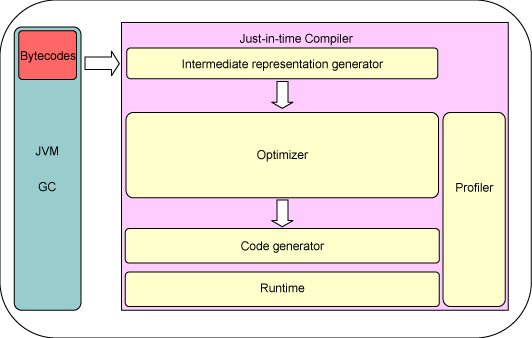
\includegraphics[width=0.7\linewidth]{jvmjit}
	\caption[Compilatore JIT]{Compilatore JIT}
	\label{fig:jit}
\end{figure}
I programmi Java vengono compilati un metodo alla volta mentre eseguono, per raggiungere performance migliori. Durante il processo viene generata una rappresentazione interna del metodo (differente dal bytecode, ma ad un livello più alto delle istruzioni macchina). Il compilatore poi esegue una serie di ottimizzazioni per migliorare la qualità e l'efficienza del codice finale e infine traduce tutto in istruzioni macchina del processore in uso. Il compilatore opera in un thread differente cosicché l'applicazione non è costretta a bloccarsi in attesa della fine della compilazione. Un framework (\texttt{Profile}) osserva il comportamento del programma per identificare i metodi eseguiti più frequentemente. 

L'eseguire la compilazione concorrentemente all'esecuzione mantiene l'indipendenza dalla piattaforma, ma ad un costo: il tempo richiesto per compilare si somma al tempo richiesto per l'esecuzione. Ci sono due soluzioni al problema:
\begin{itemize}
	\item compilare tutto il codice senza però effettuare analisi o ottimizzazioni costose (per mantenere veloce il processo). L'overhead in questo caso è talmente piccolo che è completamente recuperato dall'incremento di performance; 
	\item compilare solo metodi eseguiti veramente frequentemente (metodi \textit{hot}). L'overhead è mantenuto basso perché molte applicazioni eseguono frequentemente solamente una piccola parte del codice, quindi è sufficiente compilare quello per ottenere un significativo aumento di performance.
\end{itemize}

\subsubsection{Vantaggi}
I compilatori JIT possono analizzare l'esecuzione e identificare le situazioni che si avverano più comunemente. A partire da queste possono poi compilare il codice (anche con ottimizzazioni molto spinte) per raggiungere performance altissime. Un esempio è dato da una semplice procedura di copia di un array, \texttt{arrayCopy}. Se viene rilevato che la dimensione dell'array è praticamente costante allora è possibile generare codice ottimizzato per quella lunghezza. 

\subsubsection{Svantaggi}
Dato che è necessaria una fase di ''training'' per capire quali parti compilare, spesso le migliori performance si ottengono dopo un po'. Inoltre i metodi eseguiti frequentemente in questo periodo iniziale potrebbero non essere effettivamente quelli più significativi. Ad ogni modo le tecniche di analisi utilizzate oggigiorno eliminano il problema. 

Alcune applicazioni, però, non possono tollerare il ritardo introdotto dalla compilazione. Un esempio sono quelle da eseguire real-time.

\subsection{Compilazione Ahead-of-time}
La compilazione AOT la trasformazione in codice nativo avviene a priori, prima dell'esecuzione. Questo evita i problemi di analisi del codice e del ritardo di esecuzione, ma introduce altre problematiche. Una di queste è dovuta al caricamento dinamico delle classi. Il compilatore in questo caso non può fare nessuna assunzione riguardo a quali classi saranno caricate. Queste possono risiedere in altre macchine oppure non esistere affatto prima dell'esecuzione (con meccanismi di reflection è possibile creare classi ''al volo'', durante l'esecuzione). Questa è una grande limitazione, perché inibisce alcune delle più importanti ottimizzazioni effettuate dai compilatori, tra cui l'inlining. 

Il codice deve quindi essere generato con tutti i riferimenti non risolti. Durante l'esecuzione ogni riferimento utilizzato è aggiornato con il suo valore reale. Questo può comportare una penalità nella prima esecuzione, perché tutti i riferimenti sono sconosciuti, ma le esecuzioni successive non soffriranno di ritardi.

Compilare tutto il codice può non essere una buona scelta: il codice nativo occupa generalmente più spazio, e molti metodi sono utilizzati così raramente che la loro compilazione non porta benefici. Tuttavia invocare metodi interpretati da metodi compilati (o viceversa) richiede molto più tempo che invocare metodi interpretati da metodi interpretati. Un compilatore JIT può risolvere il problema al volo, ma uno AOT deve selezionare attentamente cosa compilare e cosa no, a priori. 

\subsubsection{Vantaggi}
Il codice AOT, sebbene più lento di quello JIT, è molto più veloce del codice interpretato. Inoltre l'incremento di performance si ottiene più velocemente, perché non si devono compilare al volo metodi eseguiti frequentemente. Le applicazioni real-time, in particolare, traggono numerosi benefici da questo approccio. Le performance sono migliori e più deterministiche rispetto a JIT. 

\subsection{Confronto}
Figura~\ref{fig:performanceaotvsjit} mostra un confronto basato sulle performance. 
\begin{figure}[h]
	\centering
	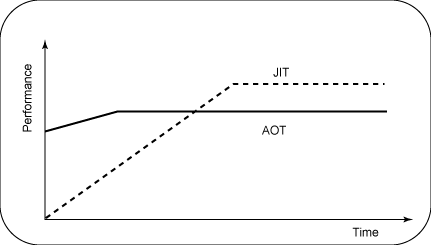
\includegraphics[width=0.7\linewidth]{performanceaotvsjit}
	\caption[Confronto di performance]{Confronto di performance}
	\label{fig:performanceaotvsjit}
\end{figure}

Inizialmente JIT è molto peggiore, perché tutti i metodi sono interpretati. Man mano che vengono compilati però le prestazioni migliorano fino a superare AOT e a raggiungere un picco. AOT, d'altra parte, ha un inizio migliore e si stabilizza più velocemente, ma ad un livello più basso. Nessuna tecnica è adatta per tutti gli scenari: l'una è più forte dove l'altra è più debole. Per le applicazioni real-time, dove l'importante è il determinismo e la prevedibilità, AOT è molto più adatto perché presenta meno variabilità nelle prestazioni.
	
	%bibliography
	\newpage
	\nocite{*}
	\printbibliography 
	
\end{document}